\documentclass[pdf]{beamer}
\usepackage{graphicx}
\usepackage{pgfpages}
%\setbeameroption{show only notes}
\mode<presentation>{}
\title{InputFinder: Reverse Engineering Closed Binaries using Hardware Performance Counters}
\author[shortname]{Bogdan Copos \inst{1} \and Praveen Murthy \inst{2}}
\institute[shortinst]{\inst{1} University of California, Davis \and \inst{2} Fujitsu Laboratories of America}
\date{}

\begin{document}

% TITLE
\begin{frame}
	\titlepage
\end{frame}

% INTRODUCTION
\begin{frame}{Introduction}
\begin{itemize}
\item Dynamic program analysis techniques necessitate test suites
\item Test suite availability and completeness issues
\item Analysis dependencies:
	\begin{itemize}
	\item platform
	\item architecture
	\item binary format
	\item source code availability
	\item ...
	\end{itemize}
\end{itemize}
\end{frame}

% BACKGROUND
%% BLACK FUZZING
\begin{frame}{Background}
\framesubtitle{\textit{Fuzzing}}
\textit{Black-box fuzzing} 
\begin{itemize}
\item Randomly generated input
\item Advantages
	\begin{itemize}
	\item easy to implement
	\item previous success
	\end{itemize}
\item Disadvantages
	\begin{itemize}
	\item poor code coverage
	\item slow
	\end{itemize}
\end{itemize}
\vspace{\baselineskip}
\end{frame}


%% WHITE FUZZING
\begin{frame}{Background}
\framesubtitle{\textit{Fuzzing}}
\textit{White-box fuzzing} 
\begin{itemize}
\item Systematically generated input
\item Advantages
	\begin{itemize}
	\item improved effectiveness
	\end{itemize}
\item Disadvantages
	\begin{itemize}
	\item limitations of constraint solver (if symbolic execution is used)
	\item source code dependencies (if instrumentation is used, i.e. afl-fuzz)
	\end{itemize}
\end{itemize}
\vspace{\baselineskip}
\end{frame}

%% SYMBOLIC EXECUTION
\begin{frame}{Background}
\framesubtitle{\textit{Symbolic Execution}}
\begin{itemize}
\item Execution of a program with symbols as input
\item Build path conditions
\item Advantages
	\begin{itemize}
	\item code coverage
	\item good results
	\end{itemize} 
\item Disadvantages
	\begin{itemize}
	\item Constraint-solver limitations
		\begin{itemize}
		\item non-linear constraints
		\item scalability (path explosion)
		\end{itemize}
	\end{itemize}
\item \textit{Concolic execution}
\end{itemize}
\end{frame}
\note{A condition on the input symbols such that if a path is feasible its path-condition is satisfiable}

\begin{frame}{DARPA Cyber Grand Challenge}

\textbf{Mission}: Design and build autonomous security systems which are capable of finding and patching vulnerabilities in unknown, closed source binaries.

\end{frame}
\note{This work started while working on a system for the DARPA Cyber Grand Challenge. The mission was to build fully autonomous systems capable of finding and patching vulnerabilities vulnerabilities in unknown, stripped, closed source binaries.}

\begin{frame}{DARPA Cyber Grand Challenge}
\begin{itemize}
\item Architecture (32 bit, x86)
\item Binary format
\item System calls
	\begin{itemize}
	\item \textit{allocate()}
	\item \textit{deallocate()}
	\item \textit{terminate()}
	\item \textit{fdwait()}
	\item \textit{random()}
	\item \textit{receive()}
	\item \textit{transmit()}
	\end{itemize}
\item No standard libraries 
\end{itemize}
\end{frame}
\note{The binary format was similar to ELF although there were some differences. For example, no dynamic linking was allowed. Also, the binaries were x86 32 bit but did not use the UNIX system calls. Instead there were 7 system calls available. This also means that the binaries did not use the GNU standard libraries.}

% PROBLEM STATEMENT
\begin{frame}{Problem Statement}
\textcolor{red}{Platform, architecture, format, source-code} \textbf{independent} method for generating input for programs.
\end{frame}

%EXPLANATION
\begin{frame}{}
Programs will normally
\begin{itemize}
\item read input
\pause
\item \textcolor{red}{validate input}
\pause
\item process
\pause
\item change state (possibly)
\pause
\item provide output (possibly)
\end{itemize}
\end{frame}

\begin{frame}{Validation}
The processor performs \textcolor{red}{additional} work during input validation.
\pause
\vspace{\baselineskip}

The amount of work varies based on the validity of the input.

\pause
\vspace{\baselineskip}

E.g.: \textit{strcmp()} stops at first character mismatch.
\pause

\vspace{\baselineskip}

\textbf{Use this observation to identify valid input}

\end{frame}
\note{The amount of work done by the processor during the validation process depends on the validity of the input. For example, when using GLIBC's strcmp function, the more valid characters the input has, the more work the processor will perform. This information can be used to identify when the program is given valid input. For the purpose of this work, we defined valid input as input that passes the validation mechanism. Valid input may be benign but it may also cause the program to crash.}


% PROPOSE APPROACH
\begin{frame}{Proposed Approach}
Leverage information exposed by the hardware [performance counters] during the program's execution
\vspace{\baselineskip}
\begin{enumerate}
\item Analyze the number of instructions retired to incrementally build input strings
\item Use discovered input and dynamically generated traces to identify the expected protocol
\end{enumerate}
\end{frame}
\note{Our approach leverages information exposed by the hardware performance counters during the program's execution. Similar results can be obtained by using instrumentation, however, experimental results show that instrumentation is significantly slower. The only overhead of using hardware counters is in reading the values from the counters. There are two main components. The first analyzes the number of instructions retired to incrementally build input strings. Second, using the discovered input and execution traces, we identify the expected protocol.}


% ASSUMPTIONS
\begin{frame}{}
Assumptions:
\begin{itemize}
\item Number of instructions retired vary based on the validity of the input.
\pause
\item Validation occurs in user-space
\pause
\item Most printable characters are not valid at a given input string index.
\pause
\item Input is interpreted as a string and validated in order.
\pause
\item No inter dependencies between fields of a single input.
\pause
\item Input is not altered prior to validation.
\end{itemize}
\end{frame}
\note{\tiny While our method can be a standalone tool, it is not meant to completely replace symbolic execution engines or fuzzers. We believe its strengths complement the weaknesses of other methods. That said, our approach does make some assumptions that must hold. For our approach to be successful, we make several assumptions. One assumption is that, as mentioned before, the number of instructions retired varies depending on the input and its validity. The more valid characters an input has, the more work is done by the processor during validation. We also assume that validation occurs in user-space and we can measure those instructions. Another assumption is that for a given program, for any of its input strings, the majority of the printable characters will not be valid at a given index. Currently our approach cannot handle cases where the input is not validated in order, where the input is composed of multiple fields that are inter dependent, or where the input undergoes transformations, such as hashing or encryption, before being validated.}

% METHODOLOGY
%\begin{frame}{Methodology}
%\end{frame}

% FINDING INPUT
\begin{frame}{Finding Input}
\begin{enumerate}
\item Start with an empty input string
\pause
\item Count the number of user-land instruction retired as the program is given as input each character from the set of printable characters
\pause
\item Calculate the mode number of user-land instructions 
\pause
\item Valid characters for the current index of the input are characters for which the number of user-land instructions retired is not within the range of mode +/- threshold
\pause
\item Append one of the discovered valid characters to the current input string and repeat steps 2-5 (until no more valid characters are identified).
\end{enumerate}
\end{frame}
\note{\tiny First we start with an empty input string. We do not assume any prior knowledge of the binary. The input finding process begins by testing the binary, with printable characters, one at a time, as the input. Using the UNIX perf utility, we count the number of user land instructions retired during each execution. We record these counter values and at the end, calculate the mode. This is where the "majority" rule comes into play. We assume that valid characters are characters for which the number of instructions retired is outside the range of mode +/- some threshold. Essentially, we assume that most printable characters are not valid, therefore will take the same execution path. On the other hand, valid characters will take different paths (compared to non-valid characters). The threshold is there because hardware performance counters are not perfect and from our experiments, the number of user land instructions retired can vary by 1 or 2 instructions for identical executions. To build entire valid input strings, we continue steps 2 through 5 until no more valid characters are identified.}

% FINDING INPUT ARCHITECTURE
\begin{frame}{}
\begin{figure}
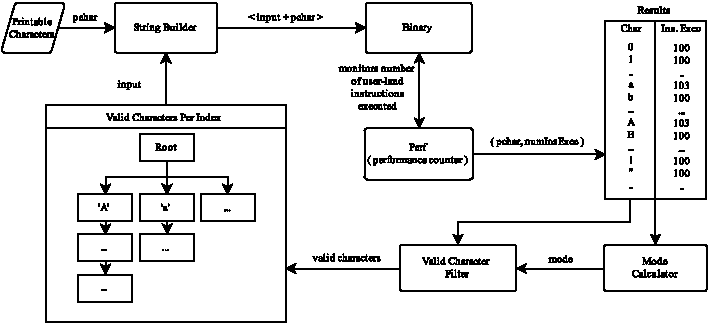
\includegraphics[scale=0.90]{../paper/architecture.pdf}
\end{figure}
\end{frame}

%FINDING INPUT SIZE
\begin{frame}{Finding Input Size}
\textbf{Idea}: Work done by processor to read input is a function of the input size and the input buffer size
\begin{enumerate}
\item Send three short inputs (e.g. 3,4,5 characters long)
\item Record delta (difference in number of instructions retired between consecutive length inputs)
\item Increase input size exponentially and send three inputs of consecutive lengths (e.g. 100,101,102 characters long)
\item Compare current deltas with expected delta
\item Repeat steps 3-4 until change is observed
\end{enumerate}

\end{frame}
\note{}

%CLASSIFYING INPUT
\begin{frame}{Classifying Input}
Determine type of accepted characters even when the program does not have predefined input/commands.

\pause
\vspace{\baselineskip}

Help fuzzers achieve better results, faster.

\end{frame}
\note{Another benefit of our method is that we can help classify the type of input a program is willing to accept. For example, consider programs which do not have a predefined set of commands or protocol. However, they only accept certain type of printable characters. Our approach is able to determine that by finding the set of acceptable characters and doing simple analysis on them. This helps fuzzers achieve better coverage faster.}

\begin{frame}{Protocol State Machine Generation}
To discover the expected protocol:
\begin{enumerate}
\item Generate every permutations of input strings
\item Discover arguments for input strings
\item Test permutations with instrumented binary
\item Compare execution traces
\end{enumerate}
\end{frame}
\note{\fontsize{4pt}{0}\selectfont To find the underlying expected protocol implemented by a given program, we first start with the input strings generated by the input finding technique described earlier. We generate all permutations of those strings, of all sizes from 2 to the number of input strings. So if we have 10 input strings, our largest permutation will be composed of 10 strings. Next, we take these permutations and while maintaining the order of the input strings, we test the strings for arguments using our input finding approach. This allows us to find cases where a given command is affected by the arguments of the previous command. One example of this is authentication. Once done, we test all permutations using an instrument binary, starting with the shortest permutations. The binary is instrumented using a PIN tool which records an execution trace. We then compare the execution traces for executions for which the last input is the same (but previous input strings differ). We break up the execution trace by input command. For example, if an execution trace reflects 3 input strings. After splitting the trace file, we will have 3 parts, one corresponding to each command. Assuming most combinations of input strings will be incorrect with respect to the expected protocol, we eliminate all execution traces where the last part is identical. More simply put, if the execution trace for the last command isn't different, nothing special happened so the permutation must be incorrect. However, if compared to other traces, the last part differs for a given permutation, the execution of the last command took a different control path and we identify that as being the correct permutation. It should be noted that similarly to our input finding approach, there is also an implicit "majority" rule, where we assume most permutations of a given length are incorrect and do not reflect the expected protocol.}

\begin{frame}{Execution Traces}
Instrument binary using PIN to record every basic block (defined by its starting address) executed in order of execution
\begin{figure}
\begin{center}
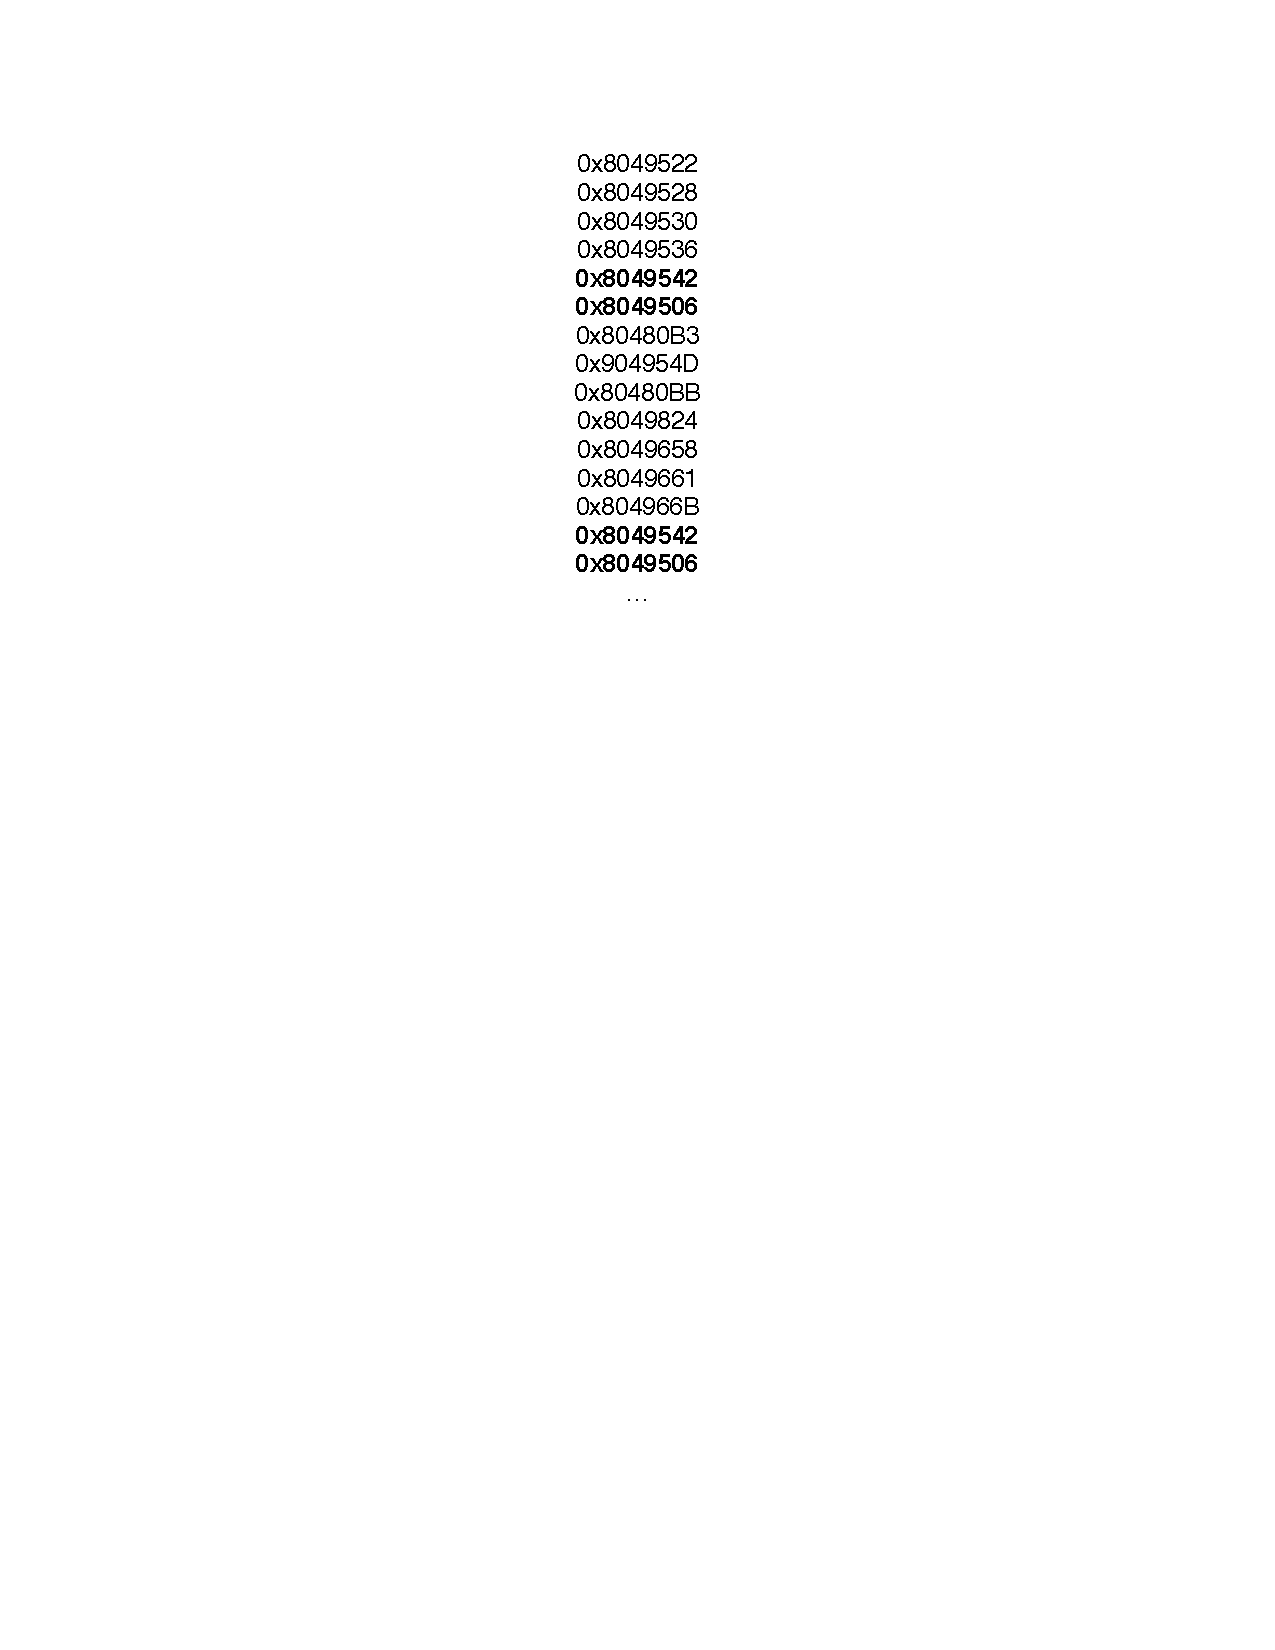
\includegraphics[scale=0.5]{../paper/traceexample.pdf}
\end{center}
\end{figure}
\end{frame}

\begin{frame}{Example}
\textbf{Valid input strings}: HELLO, AUTH, SET, CALL, BYE

\pause
\vspace{\baselineskip}

\textbf{Permutations}: [ [ HELLO, AUTH ], [ HELLO, CALL ], ... [HELLO, AUTH, SET, CALL, BYE] ]

\pause
\vspace{\baselineskip}

\textbf{Arguments}: check arguments for HELLO; send HELLO, check arguments for AUTH; send HELLO, check arguments for CALL ...

\pause
\vspace{\baselineskip}

\textbf{Compare traces}: [HELLO, AUTH] vs. [CALL, AUTH] vs. [SET, AUTH], vs. [BYE, AUTH] ... 

\end{frame}

% EVALUATION
\begin{frame}{Evaluation}
\begin{itemize}
\item 24 DARPA Cyber Grand Challenge (CGC) binaries
\item 1 cyber security interview challenge (password cracking program) 
\end{itemize}
\end{frame}


% RESULTS
\begin{frame}{Results}
\begin{table}
\scalebox{0.55}{
\begin{tabular}{|c|c|c|c|c|c|} \hline
\textbf{Binary} & \textbf{Input} & \textbf{Number of Inputs} & \textbf{Input Size} & \textbf{Crash Input} & \textbf{Protocol State Machine}\\ \hline
06459301 & yes (8 min) & 8 out of 8 & yes & no & -\\ \hline
06b71301 & no & - & yes & no & -\\ \hline
07a9a901 & - & - & yes & yes & - \\ \hline
0b32aa01 & yes (2 min) & 1 out of 1 & yes & yes & - \\ \hline
11dc8e01 & no & - & yes & no & - \\ \hline
1877a601 & yes (11 min) & 6 out of 6 & yes & no & - \\ \hline
250d1101 & yes (20 min) & 5 out of 5 & yes & no & yes \\ \hline
2eca0101 & yes (42 min) & 7 out of 7 & no & no & - \\ \hline
37e97201 & yes (38 min) & 6 out of 6 & yes & no & - \\ \hline
3dcf1a01 & yes (6 min) & 6 out of 6 & yes & yes & - \\ \hline
48b9cf01 & yes (50 min) & 9 out of 9 & yes & no & - \\ \hline
65884701 & no & - & no & no & - \\ \hline
701b7301 & - & - & yes & no & - \\ \hline
7262d006 & yes (5 min) & 4 out of 5 & yes & no & - \\ \hline
7fa39f01 & no & - & yes & yes & - \\ \hline
b8993403 & yes (12 min) & 1 out of 1 & yes & no & - \\ \hline
badd9e01 & no & - & yes & no & - \\ \hline
caea9c01 & no & - & yes & no &  -\\ \hline
cc366801 & yes (60 min) & 10 out of 10& no & no & - \\ \hline
d476cd01 & no & - & yes & no & - \\ \hline
df9df201 & no & - & yes & no & - \\ \hline
e7cd3901 & - & - & no & yes & - \\ \hline
f14eb101 & yes (53 min) & 11 out of 11 & no & no & yes \\ \hline
f658d801 & yes (2 min) & 1 out of 4 & yes & no & - \\ \hline
interview challenge & yes (2 min) & 1 out of 1 & yes & - & - \\ \hline
\end{tabular}}
\end{table}
\end{frame}
\note{The table describes the results of our evaluation. The \textit{Input} column describes whether our approach was able to discover valid input strings. As previously mentioned, some binaries did not have any predefined input strings (hence such binaries are marked by the \textit{-} in this column). The \textit{Number of Inputs} column describes how many input strings our method discovered out of the total number of input strings defined by the binary.}

\begin{frame}{Results}
\begin{itemize}
\item CGC
	\begin{itemize}
	\item Binaries with well defined input: 21 out of 24
	\item Found some input strings 13 out of 21 (62\%)
	\item Found all input strings 11 out of 13 (85\%)
	\end{itemize}
\item Interview challenge password cracked
\end{itemize}
\end{frame}

\begin{frame}{Case Study}
\framesubtitle{\textit{250d1101}}


Binary implements a simple protocol which allows the user to perform base 64 encoding/decoding and utilize an obfuscation scheme.

\pause
\vspace{\baselineskip}

The protocol dictates that the user must first authenticate before being able to execute any commands.

\vspace{\baselineskip}
\pause

\begin{itemize}
\item 5/5 input strings discovered
\item Correct protocol identified, including hidden authentication backdoor
\end{itemize}
\begin{figure}
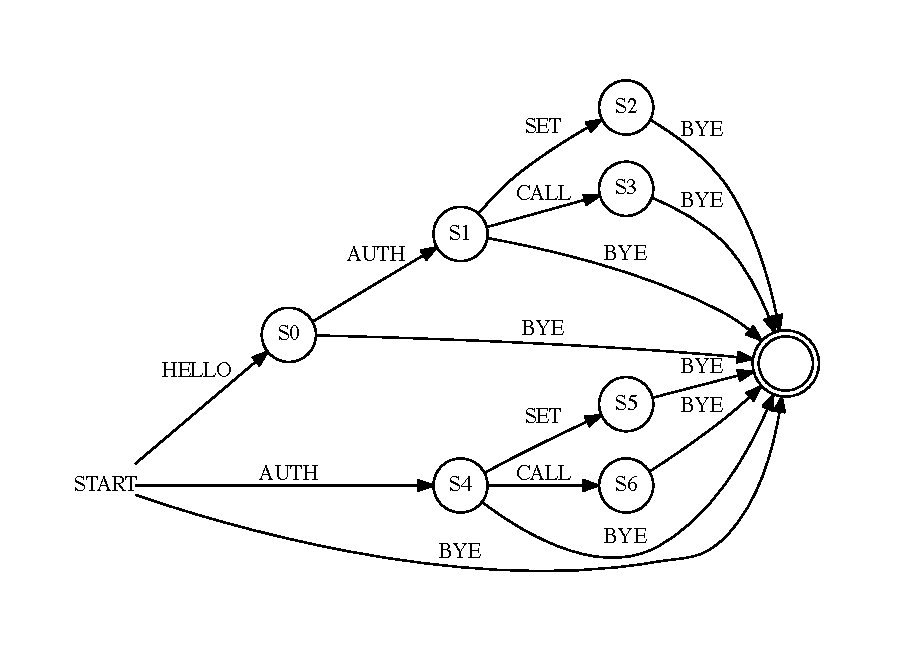
\includegraphics[scale=0.35]{../paper/protocoldiagram.pdf}
\end{figure}
\end{frame}
\note{The user must first authenticate themselves before being able to perform any actions. The authentication process begins with the user sending the HELLO command to which the program responds with a randomly generated authentication token. The user can use that token to authenticate themselves using the provided token. Once authenticated, the user can use the SET and CALL commands to ... and the BYE command to terminate the program.}

% LIMITATIONS
%\begin{frame}{Limitations}
%\end{frame}

% FUTURE WORK
\begin{frame}{Future Work}
\begin{itemize}
\item Eliminate the ``majority" constraint

\vspace{\baselineskip}
\pause

\item Use hardware counters for protocol state machine generation (vs. PIN instrumentation)
\end{itemize}
\end{frame}
\note{One of the biggest weaknesses of our approach is the majority constraint. We'd like to not have to assume that most characters are invalid for a given index of a string. Similarly we'd like to avoid assuming that most permutations of input commands are incorrect. We plan on exploring other events which can be measured using hardware counters to eliminate these constraints. Also, we'd like to use hardware counters for protocol state machine generation, to avoid the overhead of PIN instrumentation.}

% THANK YOU
\begin{frame}
\begin{center}
Thank you!

\vspace{1in}

Questions?
\end{center}
\end{frame}

% TODO:
% - citations (challenge interview)


\end{document}